\section{PS1b: Application of LFSR with SFML library}\label{sec:ps1b}
\graphicspath{{ps1b}}
\subsection{Discussion:}\label{sec:ps1b:disc}
This assignment branched off of the work finished in part (a). The linear feedback shift register was implemented in a way to encode images. The LFSR provides the perception of randomness and almost the trapdoor mechanism of encryption. The program steps through each pixel in the respective image and uses the object oriented nature of LFSR to reconfigure each component of the RGB based on the seed provided in the command line argument. As shown in the images below, the image can be encoded and decoded without any loss of information. 
    
\subsection{Key algorithms, Data structures and OO Designs used in this Assignment:}\label{sec:ps1b:kdo}

I used The Vector STL in the LFSR as it is much easier to use and I felt flexible in it. I used Two windows and two sprites for showing the difference between the normal cat image and the encoded and decoded image. 
 

\subsection{Images used:}\label{sec:ps1b:img}
\begin{figure}[h]
    \centering
    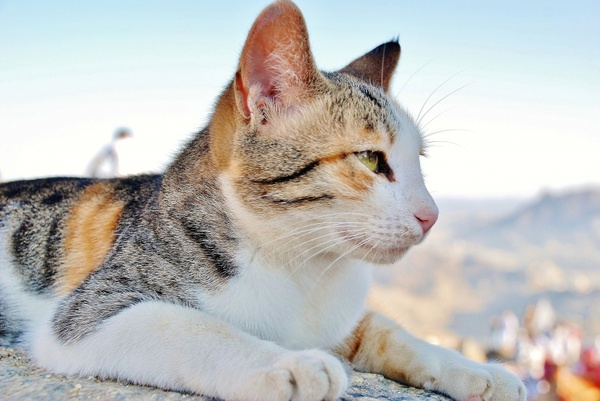
\includegraphics[width=0.45\textwidth]{projectPictures/cat.png}
    \caption{Cat Image}
    \label{fig:mesh1}
\end{figure}

\subsection{What I learned :}\label{sec:ps1b:learn}

In this assignment it was very eye opening and enlightening. First we spent the time to develop our own library for LFSR and then promptly created an application that puts the technology into work. The assignment both exercised my understanding of the SFML library and also how to utilize opaque object design. 


\subsection{Acknowledgements :}\label{sec:ps1b:ack}
\begin{itemize}
    \item \url{https://www.sfml-dev.org/tutorials/2.5/}
\end{itemize}
\newpage

\subsection{Codebase}\label{sec:ps1b:code}

\colorbox{pink}{\textbf{Makefile:}} \newline \textbf{This Makefile is contains no lint but it includes the flags as well as it is extension of the ps1a Makefile.}

\lstinputlisting[language=Make]{ps1b/Makefile}



\colorbox{pink}{\textbf{PhotoMagic.cpp:}} \newline \textbf{This file is the main file where the reading and writing also the encoding and decoding of the image takes place. This file gives the output in two windows. Input window and output window of the file.}
\lstinputlisting{ps1b/PhotoMagic.cpp}


\colorbox{pink}{\textbf{FibLFSR.h:}}
\lstinputlisting{ps1b/FibLFSR.h}

\colorbox{pink}{\textbf{FibLFSR.cpp:}}
\lstinputlisting{ps1b/FibLFSR.cpp}


\subsection{Output:}\label{sec:ps1b:output}
\begin{figure}[h]
    \centering
    
\includegraphics[width=1\textwidth]{projectPictures/encode.png}
    \caption{Encoded Image}
    \label{fig:encode}
\end{figure}
\begin{figure}[h]
    \centering
    \includegraphics[width=1\textwidth]{projectPictures/Decode.png}
    \caption{Decode Image}
    \label{fig:decode}
\end{figure}


